\section{Energy scale calibration}

\subsection{Resolution Scans}
The spectra obtained for americium (figure \ref{fig:scan:americium}) and iron
(figure \ref{fig:scan:iron}) are presented for different gains and voltages. A
guassian is fitted to the marked region of interest (ROI) and the obtained channel number as well as
full-width half-maximum (FWHM) in channels are denoted in the figure.

The obtained paramaters from the fit are plotted in figures
\ref{fig:resolution:americium} and \ref{fig:resolution:iron} for americium and
iron respectively. The uncertainties are propagated from the fit. Additional the
FWHM contains a \SI{10}{\percent} systematic uncertainty due to the dependency
on choosing the corresponding ROI.

\begin{figure}[htb]
  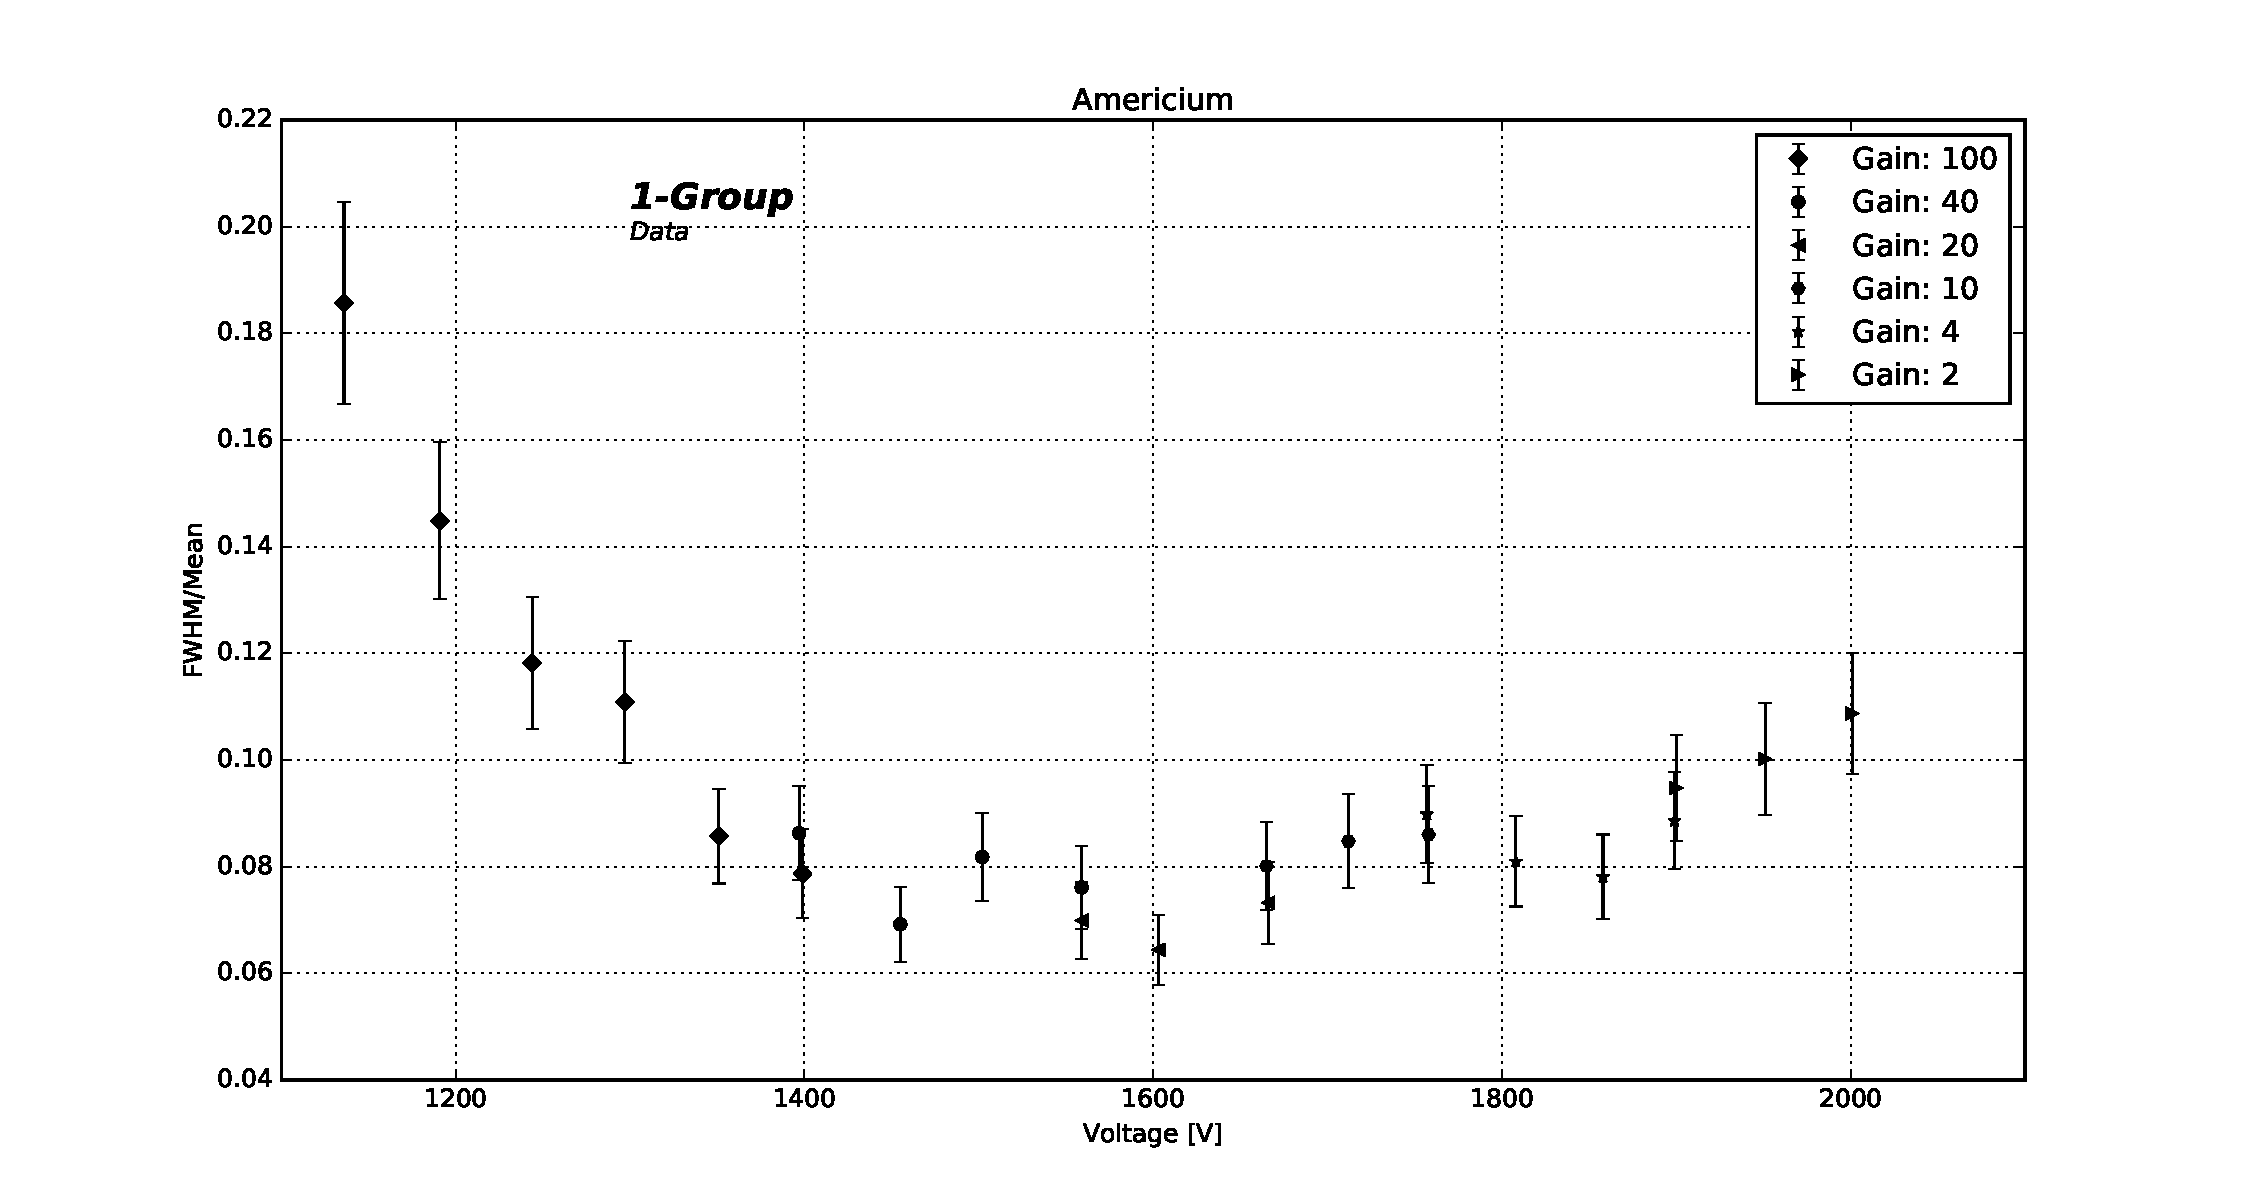
\includegraphics[width=\linewidth]{graphics/americium_scan}
  \caption{Americium scan}
  \label{fig:resolution:americium}
\end{figure}

\begin{figure}[htb]
  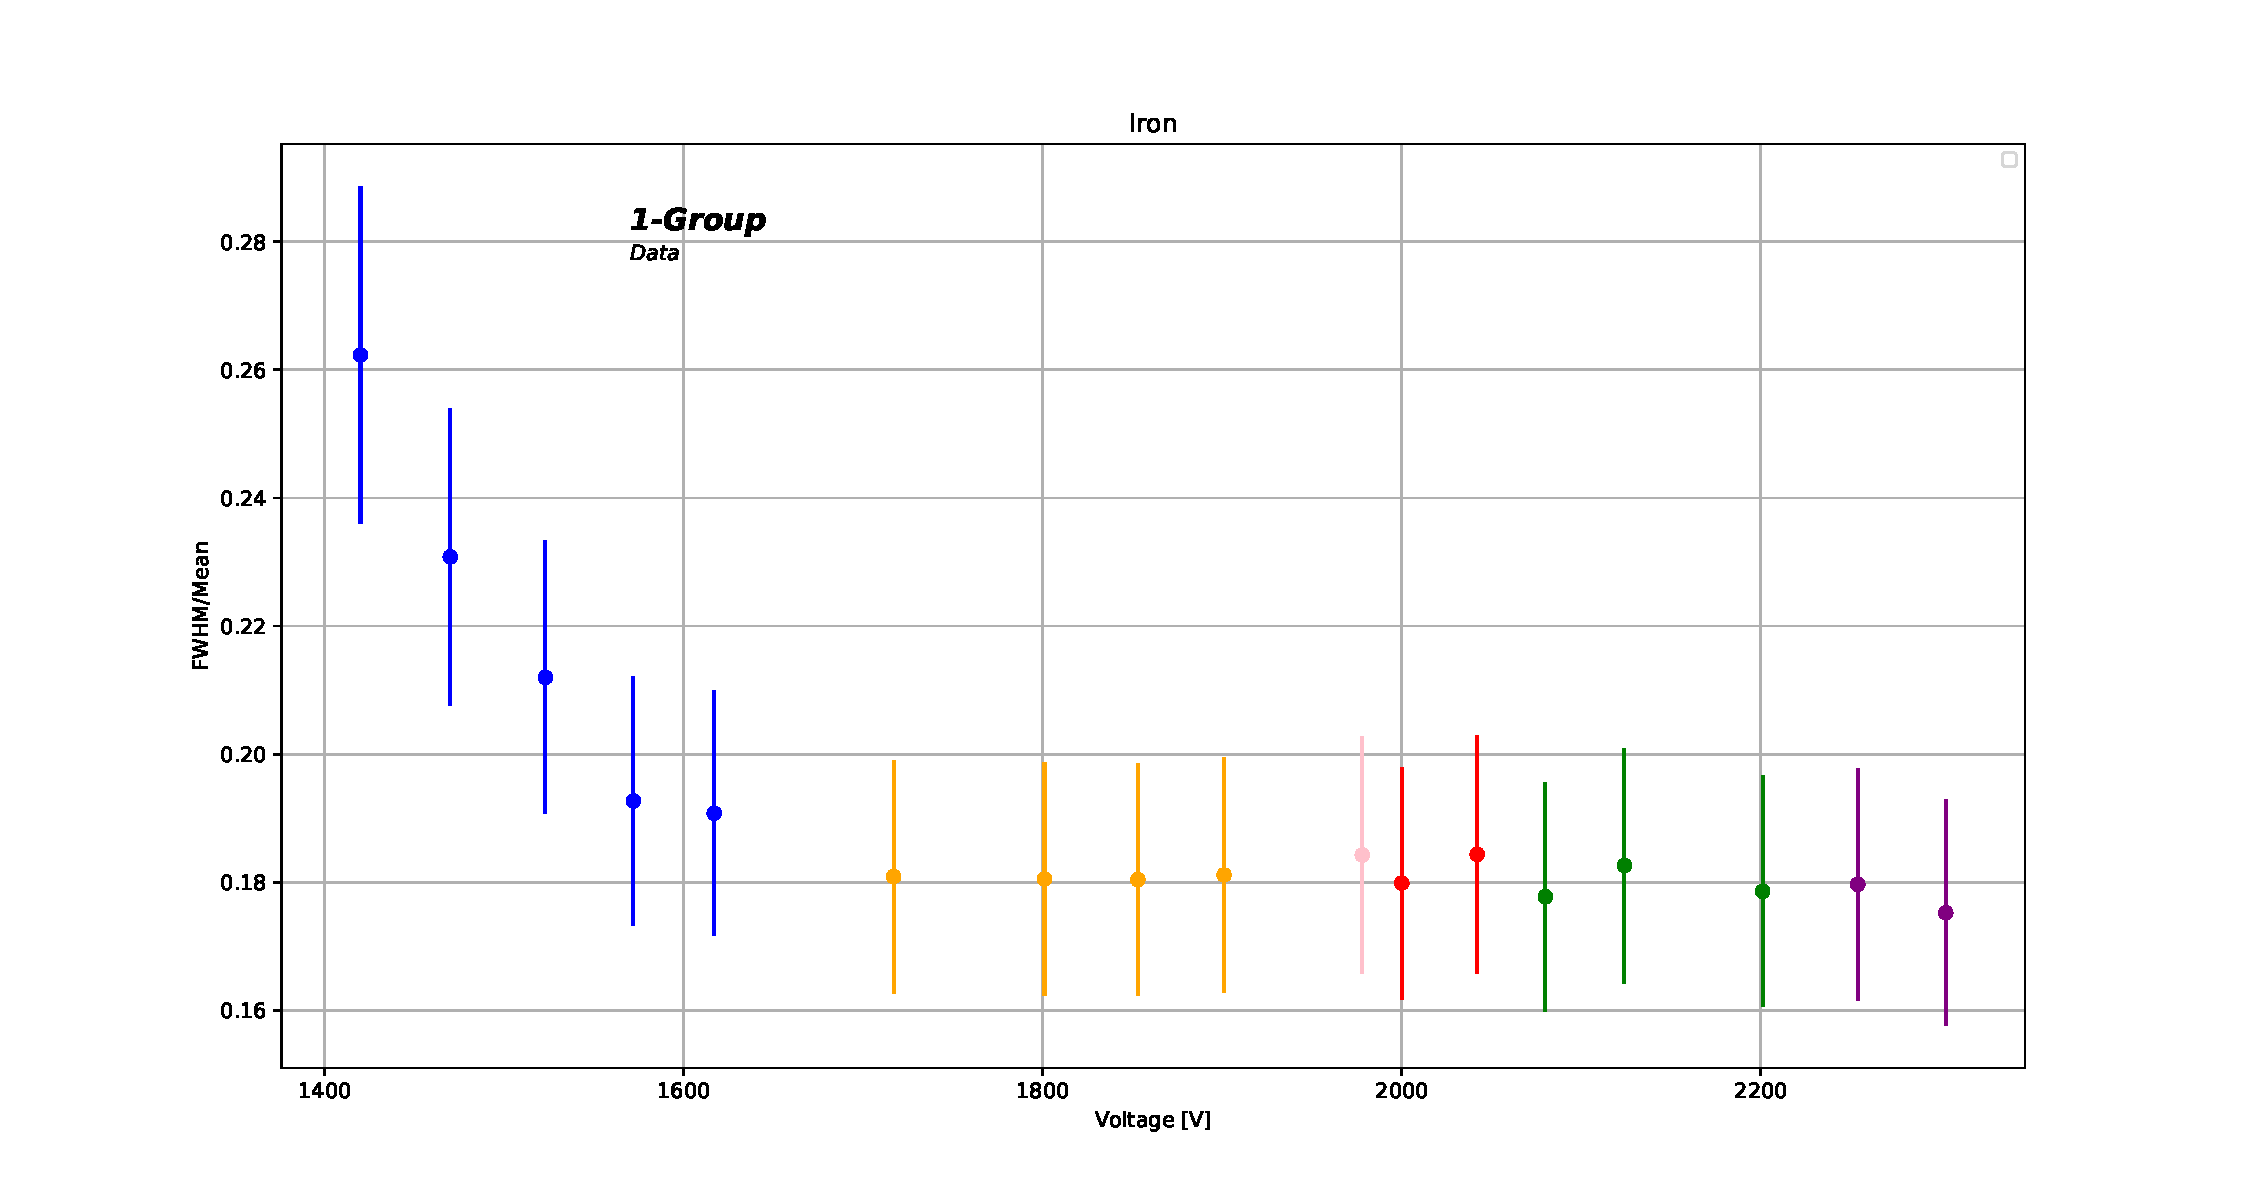
\includegraphics[width=\linewidth]{graphics/iron_scan}
  \caption{Iron scan}
  \label{fig:resolution:iron}
\end{figure}


  \begin{figure}[htb]
  \foreach \n [count=\i] in {%
    am_100_1136,
    am_100_1191,
    am_100_1244,
    am_100_1297,
    am_100_1351,
    am_100_1399,
    am_40_1397,
    am_40_1455,
    am_40_1502,
    am_40_1559}{
   \begin{subfigure}{.5\linewidth}
        \centering
         \includegraphics[width=\linewidth]{graphics/\n}
        \caption{\detokenize\expandafter{\n}}
      \end{subfigure}
    }
  \end{figure}
  \begin{figure}[htb]\ContinuedFloat
  \foreach \n [count=\i] in {%
    am_20_1559,
    am_20_1603,
    am_20_1666,
    am_10_1665,
    am_10_1712,
    am_10_1758,
    am_4_1757,
    am_4_1808,
    am_4_1858,
    am_4_1899}{
   \begin{subfigure}{.5\linewidth}
        \centering
         \includegraphics[width=\linewidth]{graphics/\n}
        \caption{\detokenize\expandafter{\n}}
      \end{subfigure}
    }
\end{figure}
  \begin{figure}[htb]\ContinuedFloat
  \foreach \n [count=\i] in {%
    am_2_1900,
    am_2_1951,
    am_2_2001} {
   \begin{subfigure}{.5\linewidth}
        \centering
         \includegraphics[width=\linewidth]{graphics/\n}
        \caption{\detokenize\expandafter{\n}}
      \end{subfigure}
    }
    \caption{Scan for different gains and voltages for Americium.}
    \label{fig:scan:americium}
\end{figure}

  \begin{figure}[htb]
  \foreach \n [count=\i] in {%
fe_100_1420,
fe_100_1470,
fe_100_1523,
fe_100_1572,
fe_100_1617,
fe_100_1717,
fe_40_1717,
fe_40_1801,
fe_40_1853,
fe_40_1901}{
   \begin{subfigure}{.5\linewidth}
        \centering
         \includegraphics[width=\linewidth]{graphics/\n}
        \caption{\detokenize\expandafter{\n}}
      \end{subfigure}
    }
  \end{figure}
  \begin{figure}[htb]\ContinuedFloat
  \foreach \n [count=\i] in {%
fe_20_1901,
fe_20_1978,
fe_10_1978,
fe_10_2000,
fe_10_2042,
fe_10_2080,
fe_4_2080,
fe_4_2124,
fe_4_2201}{
   \begin{subfigure}{.5\linewidth}
        \centering
         \includegraphics[width=\linewidth]{graphics/\n}
        \caption{\detokenize\expandafter{\n}}
      \end{subfigure}
    }
\end{figure}
  \begin{figure}[htb]\ContinuedFloat
  \foreach \n [count=\i] in {%
fe_2_2201,
fe_2_2254,
fe_2_2303}{
   \begin{subfigure}{.5\linewidth}
        \centering
         \includegraphics[width=\linewidth]{graphics/\n}
        \caption{\detokenize\expandafter{\n}}
      \end{subfigure}
    }
    \caption{Scan for different gains and voltages for Iron.}
    \label{fig:scan:iron}
\end{figure}
